%\documentclass{article} % One-column default
\documentclass[twocolumn, switch]{article} % Method A for two-column formatting

\usepackage{preprint}

\usepackage{caption}
\usepackage{xcolor}

\RequirePackage{rotating}
\newif\ifturnofflinenums
\let\savesidewaystable\sidewaystable
\let\savesidewaysfigure\sidewaysfigure
%% turns off line numbers in rotated tables and figures, aesthetic consideration,
%% not necessary.
\def\sidewaystable{\turnofflinenumstrue\savesidewaystable\centering}
\def\sidewaysfigure{\turnofflinenumstrue\savesidewaysfigure\centering}

\usepackage{threeparttable}

%% Math packages
\usepackage{amsmath, amsthm, amssymb, amsfonts}

\usepackage[version=4]{mhchem}
%% Bibliography options

%% natbib <-> biblatex command conversions: 
% \citep <-> \parencite : (Smith et al. 1995)
% \citet <-> \textcite .... Smith et al. (1995) ...
% \citealp <-> \cite [bare ]  ... Smith et al. 1995 ...

\usepackage[style=authoryear-comp,maxcitenames=1,uniquename=false,giveninits=true,uniquelist=false,maxbibnames=99,sortcites=true,sorting=ynt,doi=true,isbn=false,url=false,hyperref=true,date=year]{biblatex}
% Removes default behaviour s.t. Articles do not include "in" within bibliography
\renewbibmacro{in:}{
  \ifboolexpr{%
     test {\ifentrytype{article}}%
     or 
     test {\ifentrytype{inproceedings}}%
  }{}{\printtext{\bibstring{in}\intitlepunct}}%
}
% Removes language field
\AtEveryBibitem{%
  \clearlist{language}%
}
\AtEveryBibitem{%
  \clearfield{note}%
}
\addbibresource{references.bib}

%% General packages
\usepackage[utf8]{inputenc}	% allow utf-8 input
\usepackage[T1]{fontenc}	% use 8-bit T1 fonts
\usepackage{xcolor}		% colors for hyperlinks
\usepackage[colorlinks = true,
            linkcolor = magenta,
            urlcolor  = blue,
            citecolor = cyan,
            anchorcolor = black]{hyperref}	% Color links to references, figures, etc.
\usepackage{booktabs} 		% professional-quality tables
\usepackage{nicefrac}		% compact symbols for 1/2, etc.
\usepackage{microtype}		% microtypography
\usepackage{lineno}		% Line numbers
\usepackage{float}			% Allows for figures within multicol
\usepackage{mhchem}         % For chemical formula
\usepackage{lipsum}		%  Filler text
\usepackage{graphicx}
\usepackage{url}

 %% Special figure caption options
\usepackage{newfloat}
\DeclareFloatingEnvironment[name={Supplementary Figure}]{suppfigure}
\usepackage{sidecap}
\sidecaptionvpos{figure}{c}


% Section title spacing  options
\usepackage{titlesec}
\titlespacing\section{0pt}{12pt plus 3pt minus 3pt}{1pt plus 1pt minus 1pt}
\titlespacing\subsection{0pt}{10pt plus 3pt minus 3pt}{1pt plus 1pt minus 1pt}
\titlespacing\subsubsection{0pt}{8pt plus 3pt minus 3pt}{1pt plus 1pt minus 1pt}

%%%%%%%%%%%%%%%%   Title   %%%%%%%%%%%%%%%%

\title{A Very Interesting Discovery}

% Add watermark with submission status
\usepackage{xwatermark}
% Left watermark
\newwatermark[firstpage,color=gray!60,angle=90,scale=0.32, xpos=-4.05in,ypos=0]{\href{published-url}{{\color{gray}{Manuscript submitted for publication in \textit{Highly Prestigious Journal}. Published DOI: XXXXXXXXXXXXXXXXX }}}}
% Right watermark
\newwatermark[firstpage,color=gray!60,angle=90,scale=0.32, xpos=3.9in,ypos=0]{\href{preprint-url}{\color{gray}{Preprint doi: YYYYYYYYYYYYYYYYYY}}}
% Bottom watermark
\newwatermark[firstpage,color=gray!90,angle=0,scale=0.28, xpos=0in,ypos=-5in]{*correspondence: \texttt{a.lipp18@imperial.ac.uk}}

%%%%%%%%%%%%%%%  Author list  %%%%%%%%%%%%%%%
\usepackage{authblk}
\renewcommand*{\Authfont}{\bfseries}
\author[1\thanks{\tt{a.lipp18@imperial.ac.uk}}]{Alex G. Lipp}
\author[2]{C. O. Llaborator}
\affil[1]{Department of Earth Sciences and Engineering, Imperial College London, UK}
\affil[2]{Centre for Environmental Geochemistry, British Geological Survey, Keyworth, UK}

%%%%%%%%%%%%%%    Front matter    %%%%%%%%%%%%%%
\begin{document}

\twocolumn[ % Method A for two-column formatting
  \begin{@twocolumnfalse} % Method A for two-column formatting
  
\maketitle

\begin{abstract}

Lorem ipsum dolor sit amet, consectetuer adipiscing elit. Ut purus elit, vestibulum ut, placerat ac, adipiscing vitae, felis. Curabitur dictum gravida mauris. Nam arcu libero, nonummy eget, consectetuer id, vulputate a, magna. Donec vehicula augue eu neque. Pellentesque habitant morbi tristique senectus et netus et malesuada fames ac turpis egestas. Mauris ut leo. Cras viverra metus rhoncus sem. Nulla et lectus vestibulum urna fringilla ultrices. Phasellus eu tellus sit amet tortor gravida placerat. Integer sapien est, iaculis in, pretium quis, viverra ac, nunc. Praesent eget sem vel leo ultrices bibendum. Aenean faucibus. Morbi dolor nulla, malesuada eu, pulvinar at, mollis ac, nulla. Curabitur auctor semper nulla. Donec varius orci eget risus. Duis nibh mi, congue eu, accumsan eleifend, sagittis quis, diam. Duis eget orci sit amet orci dignissim rutrum. Nam dui ligula, fringilla a, euismod sodales, sollicitudin vel, wisi. Morbi auctor lorem non justo. 


\end{abstract}

\vspace{5mm}

\begin{plainlang}

Lorem ipsum dolor sit amet, consectetuer adipiscing elit. Ut purus elit, vestibulum ut, placerat ac, adipiscing vitae, felis. Curabitur dictum gravida mauris. Nam arcu libero, nonummy eget, consectetuer id, vulputate a, magna. Donec vehicula augue eu neque. Pellentesque habitant morbi tristique senectus et netus et malesuada fames ac turpis egestas. Mauris ut leo. Cras viverra metus rhoncus sem. Nulla et lectus vestibulum urna fringilla ultrices. Phasellus eu tellus sit amet tortor gravida placerat. Integer sapien est, iaculis in, pretium quis, viverra ac, nunc. Praesent eget sem vel leo ultrices bibendum. Aenean faucibus. Morbi dolor nulla, malesuada eu, pulvinar at, mollis ac, nulla. Curabitur auctor semper nulla. Donec varius orci eget risus. Duis nibh mi, congue eu, accumsan eleifend, sagittis quis, diam. Duis eget orci sit amet orci dignissim rutrum. Nam dui ligula, fringilla a, euismod sodales, sollicitudin vel, wisi. Morbi auctor lorem non justo. 


\end{plainlang}
\keywords{Science \and Data \and Fascinating Results} % (optional)
\vspace{0.35cm}

  \end{@twocolumnfalse} % Method A for two-column formatting
] % Method A for two-column formatting


%%%%%%%%%%%%%%%  Main text   %%%%%%%%%%%%%%%

\section{Introduction}

Lorem ipsum dolor sit amet, consectetuer adipiscing elit. Ut purus elit, vestibulum ut, placerat ac, adipiscing vitae, felis. Curabitur dictum gravida mauris. Nam arcu libero, nonummy eget, consectetuer id, vulputate a, magna. Donec vehicula augue eu neque. Pellentesque habitant morbi tristique senectus et netus et malesuada fames ac turpis egestas. Mauris ut leo. Cras viverra metus rhoncus sem. Nulla et lectus vestibulum urna fringilla ultrices. Phasellus eu tellus sit amet tortor gravida placerat. Integer sapien est, iaculis in, pretium quis, viverra ac, nunc. Praesent eget sem vel leo ultrices bibendum. Aenean faucibus. Morbi dolor nulla, malesuada eu, pulvinar at, mollis ac, nulla. Curabitur auctor semper nulla. Donec varius orci eget risus. Duis nibh mi, congue eu, accumsan eleifend, sagittis quis, diam. Duis eget orci sit amet orci dignissim rutrum. Nam dui ligula, fringilla a, euismod sodales, sollicitudin vel, wisi. Morbi auctor lorem non justo. 

\section{Figures} 

Figure \ref{fig:fig1} is a small photo of a duck which fits inside one column. Figure \ref{fig:fig2} is a large duck. A supplementary duck can be found in Figure S\ref{fig:SI_1}. 

\begin{figure}
  \centering
  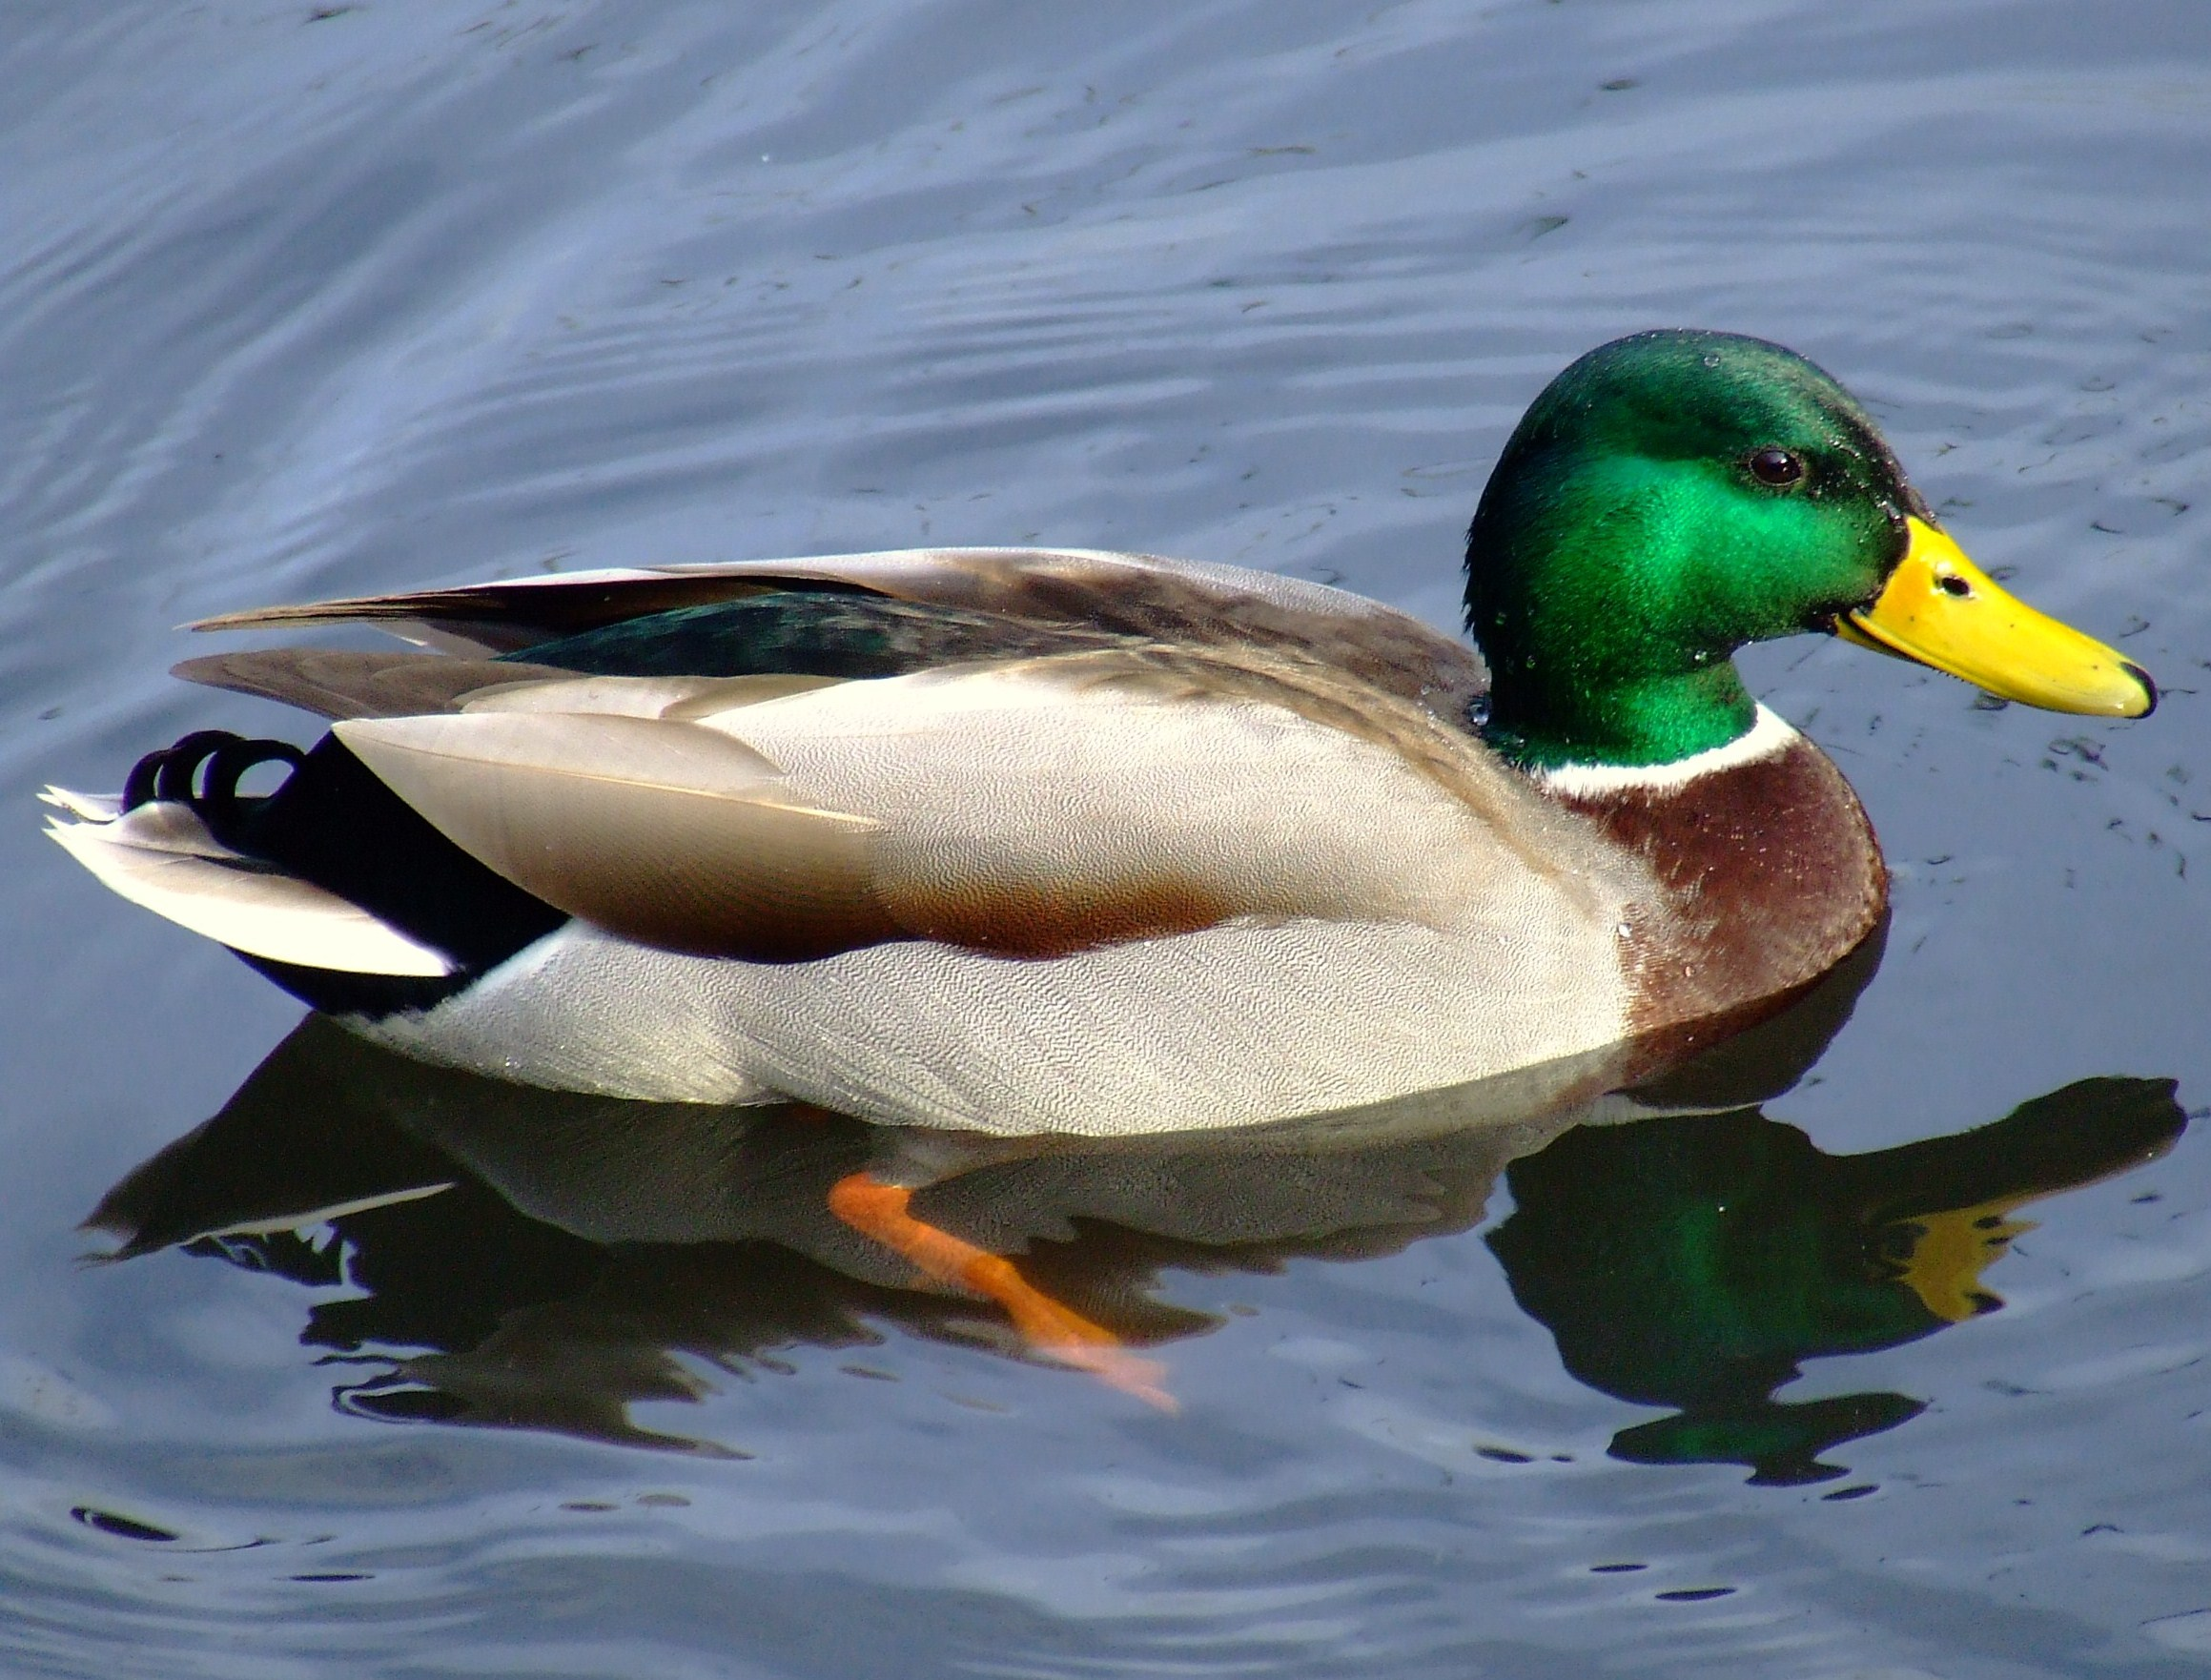
\includegraphics[scale=0.1]{duck1.jpg}
  \caption{This is a duck.}
  \label{fig:fig1}
\end{figure}

\begin{figure*}[t]
  \centering
  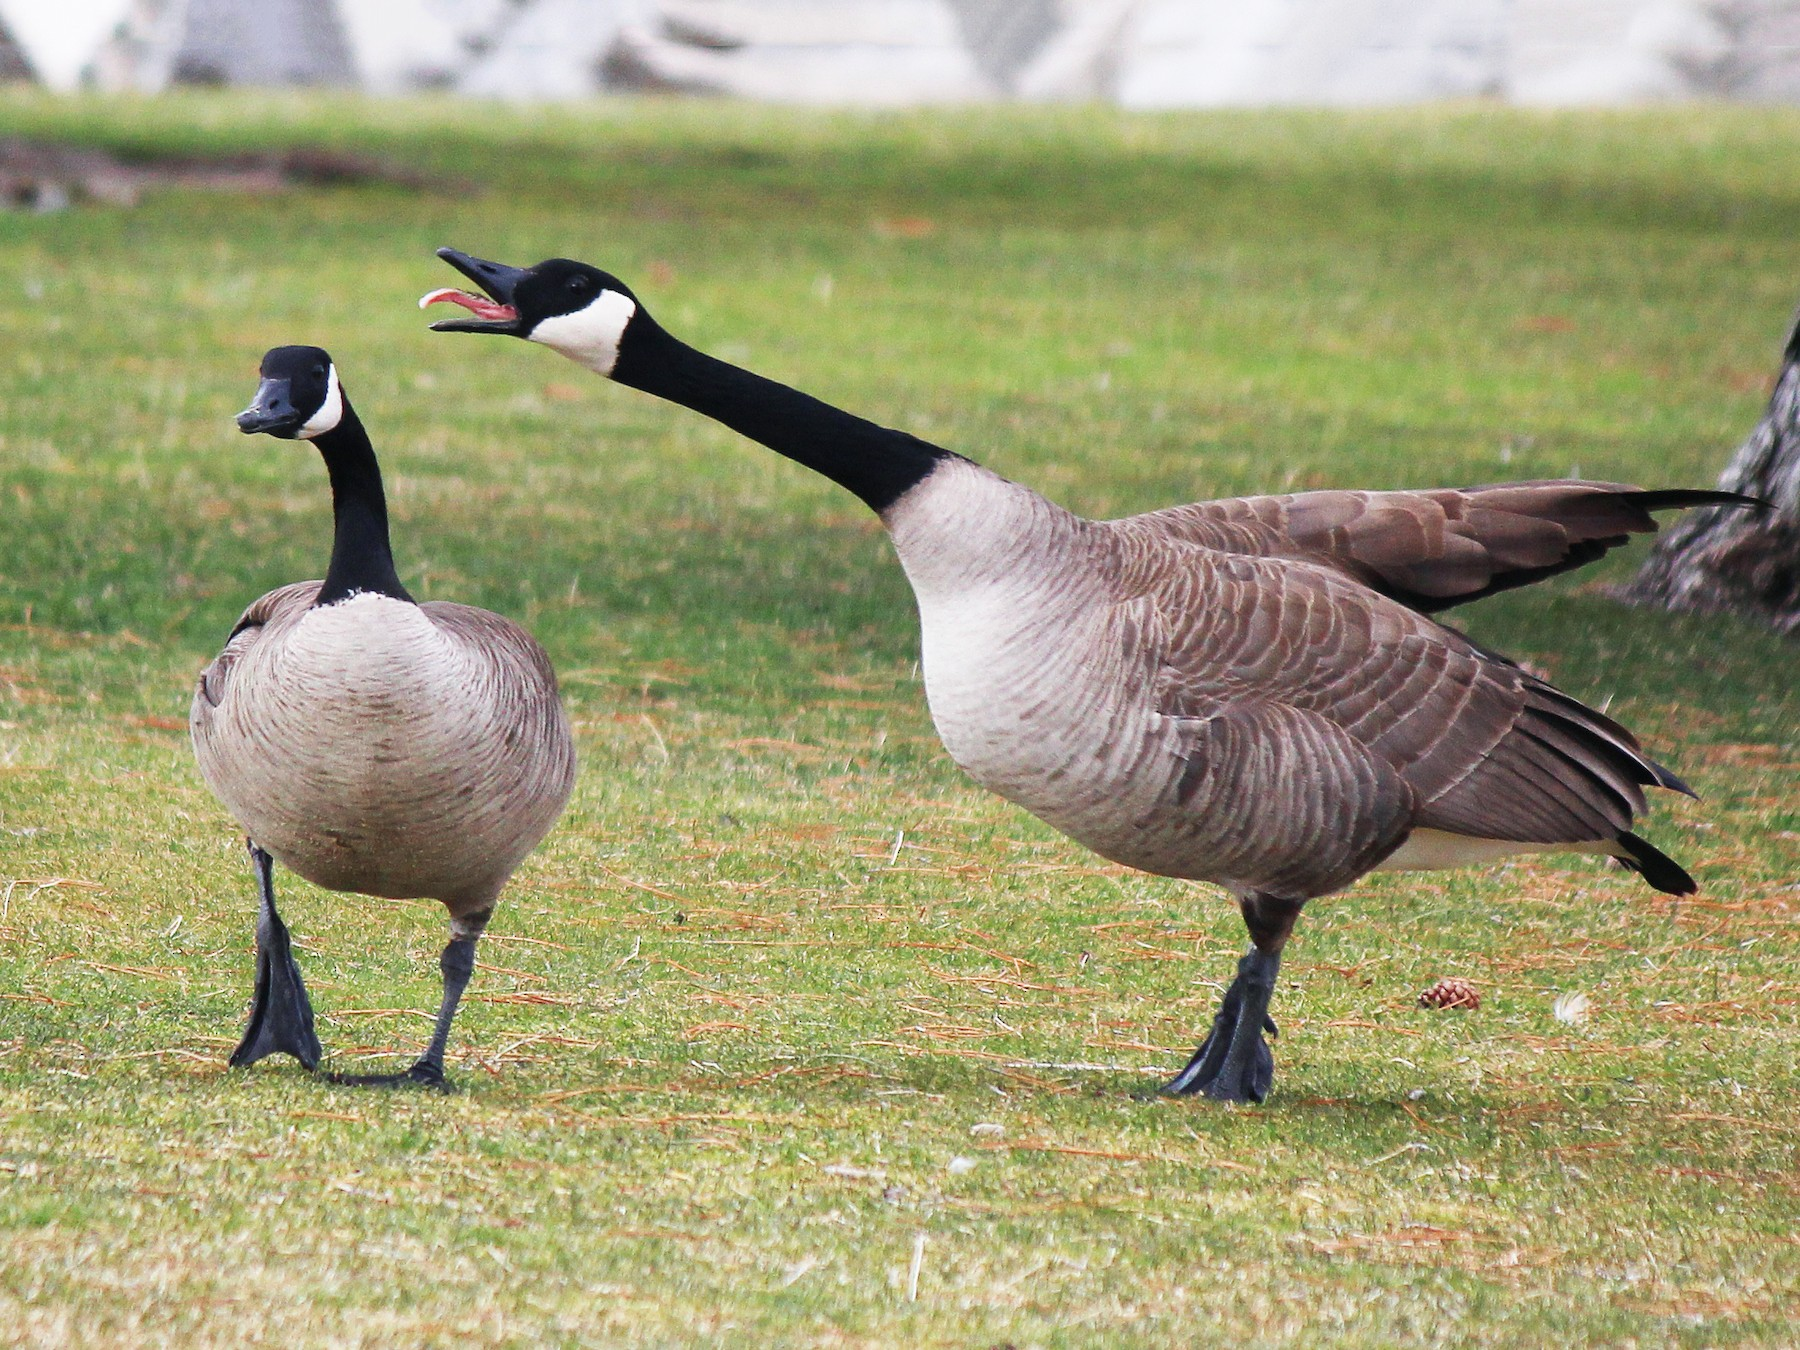
\includegraphics[scale=0.2]{goose.jpg}
  \caption{This is a large duck.}
  \label{fig:fig2}
\end{figure*}

\subsection{A subsection}

Lorem ipsum dolor sit amet, consectetuer adipiscing elit. Ut purus elit, vestibulum ut, placerat ac, adipiscing vitae, felis. Curabitur dictum gravida mauris. Nam arcu libero, nonummy eget, consectetuer id, vulputate a, magna. Donec vehicula augue eu neque. Pellentesque habitant morbi tristique senectus et netus et malesuada fames ac turpis egestas. Mauris ut leo. Cras viverra metus rhoncus sem. Nulla et lectus vestibulum urna fringilla ultrices. Phasellus eu tellus sit amet tortor gravida placerat. Integer sapien est, iaculis in, pretium quis, viverra ac, nunc. Praesent eget sem vel leo ultrices bibendum.

\subsubsection{How to do citations}

We used the fantastic data analytic methods of \textcite{aitchison_statistical_1986}. These methods are widely used in the community \autocite{von_eynatten_sediment_2016}. We also read some studies about rivers (e.g. \cite{roberts_estimating_2010}). 

\section{Maths and Tables}

This is a very important equation about rivers: 

\begin{equation}
    \frac{\partial z}{\partial t} = - v A(x)^m \left(\frac{\partial z}{\partial x} \right)^n,
    \label{eq:SPL}
\end{equation}

The results of using this equation are shown in Table \ref{tab:table}. 

\begin{table}[H]
 \caption{Sample table title}
  \centering
  \begin{tabular}{lll}
    \toprule
    \multicolumn{2}{c}{Part}                   \\
    \cmidrule(r){1-2}
    Name     & Description     & Size ($\mu$m) \\
    \midrule
    Dendrite & Input terminal  & $\sim$100     \\
    Axon     & Output terminal & $\sim$10      \\
    Soma     & Cell body       & up to $10^6$  \\
    \bottomrule
  \end{tabular}
  \label{tab:table}
\end{table}

\section{Conclusions}

Lorem ipsum dolor sit amet, consectetuer adipiscing elit. Ut purus elit, vestibulum ut, placerat ac, adipiscing vitae, felis. Curabitur dictum gravida mauris. Nam arcu libero, nonummy eget, consectetuer id, vulputate a, magna.

%%%%%%%%%%%%% Data and code availability %%%%%%%%%%%%%
\footnotesize
\section*{Data and Code Availability}
Code and data is available at \url{github.com/URL_goes_here}. 

%%%%%%%%%%%%% Acknowledgements %%%%%%%%%%%%%
\footnotesize
\section*{Acknowledgements}
The authors are extremely grateful to many people.


%%%%%%%%%%%%%%   Bibliography   %%%%%%%%%%%%%%
\normalsize

\begin{refcontext}[sorting=nyt]
\printbibliography
\end{refcontext}

%%%%%%%%%%%%  Supplementary Figures  %%%%%%%%%%%%
\clearpage 

\section*{Supporting Information}

The supporting information is very important and not an attempt to hide the methods away from scrutiny. 

Lorem ipsum dolor sit amet, consectetuer adipiscing elit. Ut purus elit, vestibulum ut, placerat ac, adipiscing vitae, felis. Curabitur dictum gravida mauris. Nam arcu libero, nonummy eget, consectetuer id, vulputate a, magna. Donec vehicula augue eu neque. Pellentesque habitant morbi tristique senectus et netus et malesuada fames ac turpis egestas. Mauris ut leo. Cras viverra metus rhoncus sem. Nulla et lectus vestibulum urna fringilla ultrices. Phasellus eu tellus sit amet tortor gravida placerat. Integer sapien est, iaculis in, pretium quis, viverra ac, nunc. Praesent eget sem vel leo ultrices bibendum.

Lorem ipsum dolor sit amet, consectetuer adipiscing elit. Ut purus elit, vestibulum ut, placerat ac, adipiscing vitae, felis. Curabitur dictum gravida mauris. Nam arcu libero, nonummy eget, consectetuer id, vulputate a, magna. Donec vehicula augue eu neque. Pellentesque habitant morbi tristique senectus et netus et malesuada fames ac turpis egestas. Mauris ut leo. Cras viverra metus rhoncus sem. Nulla et lectus vestibulum urna fringilla ultrices. Phasellus eu tellus sit amet tortor gravida placerat. Integer sapien est, iaculis in, pretium quis, viverra ac, nunc. Praesent eget sem vel leo ultrices bibendum.

\begin{suppfigure*}
  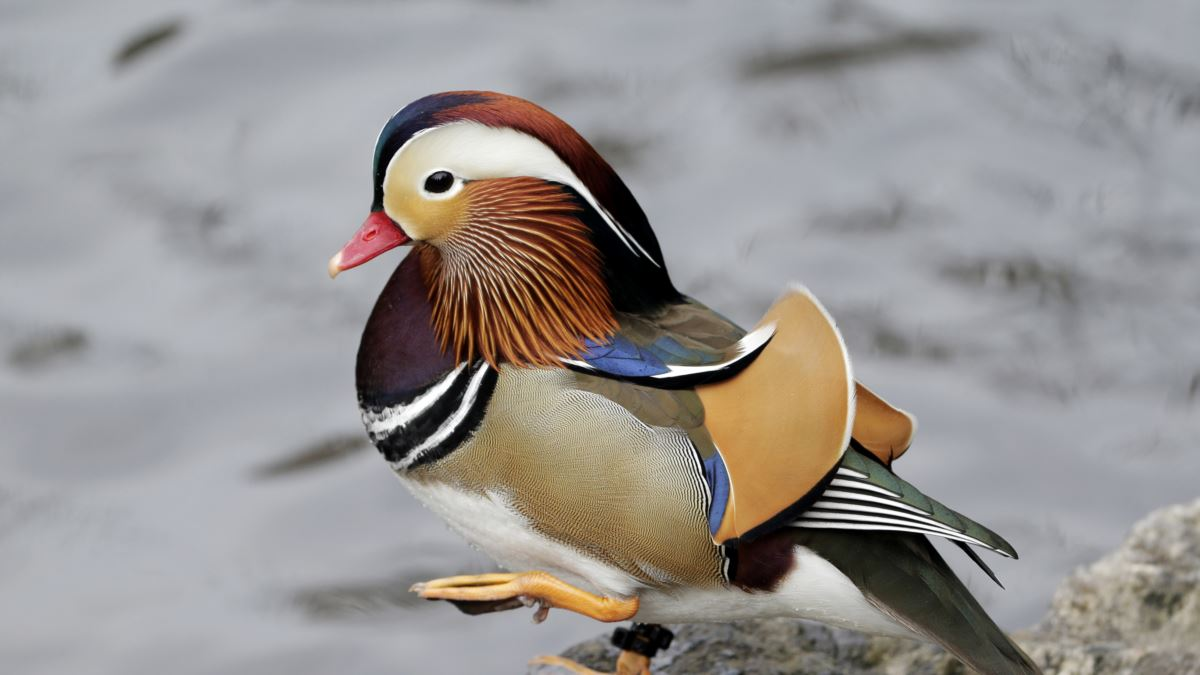
\includegraphics[scale=0.5]{duck2.jpg}
  \centering
  \caption{Supplementary duck}
  \label{fig:SI_1}
\end{suppfigure*}

%%%%%%%%%%%%%%%%   End   %%%%%%%%%%%%%%%%
\end{document}
